\begin{figure}[t]
	\centering
	\begin{subfigure}{0.31\textwidth}
		\centering
		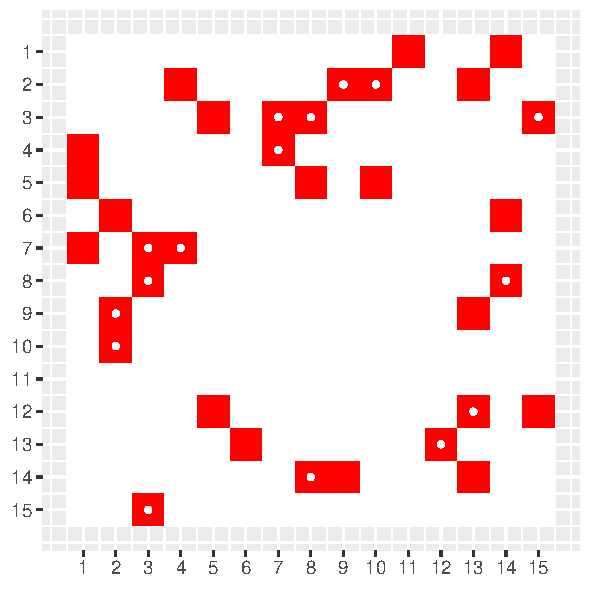
\includegraphics[width=\textwidth]{figures/penta-W.pdf}
		\caption{True Adjacency Matrix}
	\end{subfigure}
	\begin{subfigure}{0.31\textwidth}
		\centering
		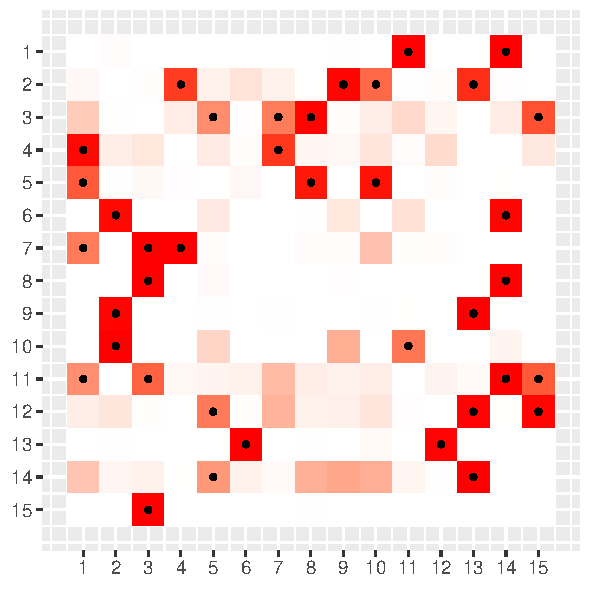
\includegraphics[width=\textwidth]{figures/P10-posterior-W.pdf}
		\caption{P10}
	\end{subfigure}
	\begin{subfigure}{0.31\textwidth}
		\centering
		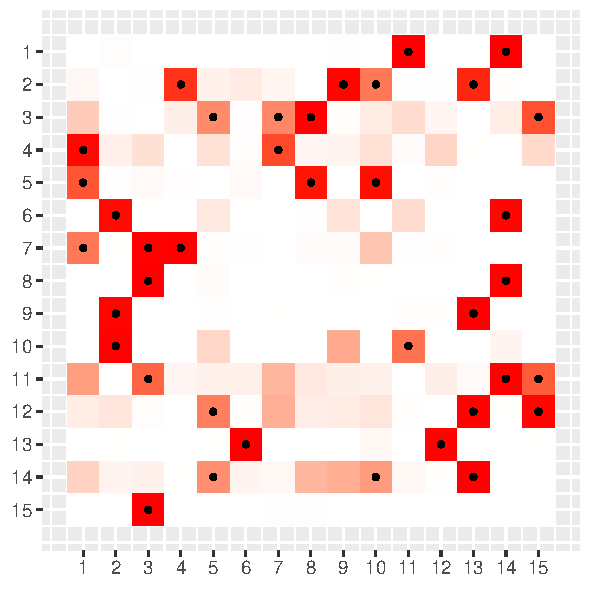
\includegraphics[width=\textwidth]{figures/P11-posterior-W.pdf}
		\caption{P11}
	\end{subfigure}
	\begin{subfigure}{0.31\textwidth}
		\centering
		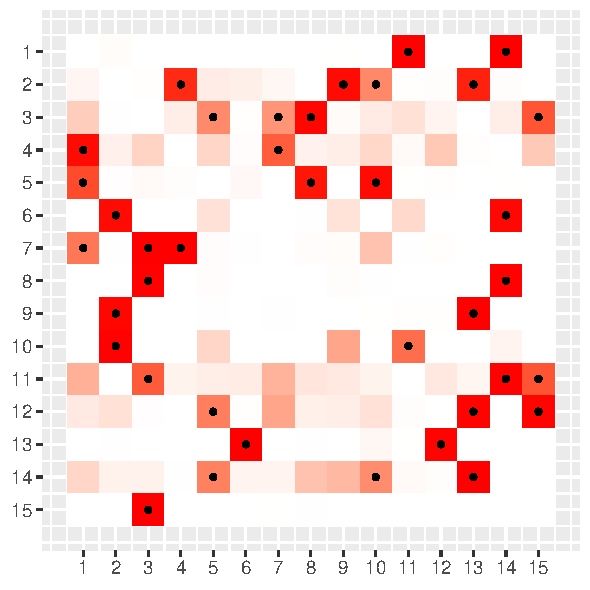
\includegraphics[width=\textwidth]{figures/P12-posterior-W.pdf}
		\caption{P12}
	\end{subfigure}
	\begin{subfigure}{0.31\textwidth}
		\centering
		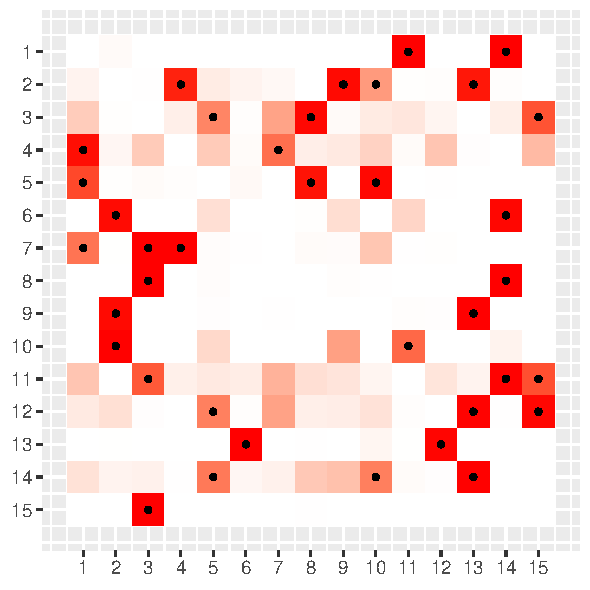
\includegraphics[width=\textwidth]{figures/P13-posterior-W.pdf}
		\caption{P13}
	\end{subfigure}
	\begin{subfigure}{0.31\textwidth}
		\centering
		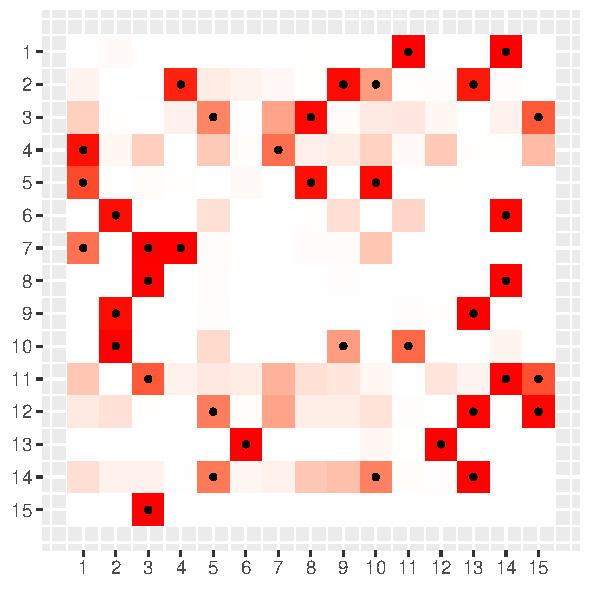
\includegraphics[width=\textwidth]{figures/P14-posterior-W.pdf}
		\caption{P14}
	\end{subfigure}
	\caption{Posterior Adjacency Matrices.}
	\label{fig:P1}
	\caption*{\footnotesize\emph{Note}: The black dots in the posterior adjacency matrices denotes the probability of entry being one exceeding $50\%$.}
\end{figure}
